% ##################################################################################################################
\chapter{The Philippines: Agent-Based Transport Simulation Model for Disaster Response Vehicles}
\label{ch:philippines}
\hfill \textbf{Author:} Elvira B. Yaneza

\editdone{This text has undergone the professional edit. Please no grammatical changes anymore! They are most-probably wrong.}

%\ahtodo{check copyrights, modify figures}

% ##################################################################################################################
This study's primary aim was adapting an agent-based traffic simulation model to assist planning agencies in determining road traffic routes for \gls{drv} in crises or disasters. After the initial disaster event period, road network management is crucial for disaster response operations, who must cope with travel demand increase. Depending on level of road damage, sections of the the road network may close. The degraded \gls{drv} road traffic routes will result in longer travel times.

The model was developed using an agent-based simulation modeling paradigm implemented through \gls{matsim}. Road traffic routes were generated using Dijkstra’s shortest path algorithm. \gls{matsim} output files stored each agent's routes, which represented traffic routes for \gls{drv}; here, each route's calculated travel time was equivalent to each agent's running time (in actual motion, while using shortest paths from source to destination). 

% ##################################################################################################################
\section{Literature Review}
Road traffic routing studies generally use different modeling approaches and shortest path algorithms. In studies using modeling, \citet[][]{LefebvreBalmer_unpub_STRC_2007} used \gls{matsim} for \gls{largescale} agent-based transport simulation, also investigating variations of Dijkstra’s algorithm and A*-algorithm. \citet[][]{SumaleeKurauchi_NSE_2006} used the Monte-Carlo simulation approach to approximate network capacity reliability, then evaluated  traffic regulation policy performance, using the Kobe city (Japan) road network. \citet[][]{Teknomo_TSSP_2008} multi-agent simulation modeling approach considered route probability as a direct simulation output, rather than input, to the network. \citet[][]{SandersSchultes_WEA_2007} outlined algorithms with faster run times than Dijkstra’s algorithm for transportation network route planning. Their study focused on successful speedup techniques in static road networks with fixed edge cost. \citet[][]{Elalouf_JSSM_2012} model incorporated joint analysis of expected route time and its variance, using dynamic-programming, shortest path algorithm as a basis for a fully polynomial time approximation scheme. 

% ##################################################################################################################
\section{Design Details And Specifications}
% ..........................................
\paragraph{Element~1: Study Area}
During Tropical Storm Washi (Sendong), areas most affected areas were those near the Cagayan de Oro river \citep[][]{Ramos_TechRep_NDRRMC_2011}. Landslides near river banks, flash floods, as well as the overflowing river and its tributaries, caused some barangays (barrios)---already damaged by Tropical Depression Shanshan (Crising)---to be swept away \citep[][]{Delrosario_TechRep_NDRRMC_2011}. The five most affected major bridges cross along the Cagayan de Oro River, connecting its two main areas, District~1 (west)and District~2 (east), in Misamis Oriental province (see Figure~\ref{fig:philippines_fig1}). The designated road network coverage has a total area of approximately 73.2\,square kilometers, including the riverside (see Figure~\ref{fig:philippines_fig3}). 

% ..........................................
\paragraph{Element~2: Road Network and Facilities}
The model involved three main entities: road network, facilities and population and is described by two variables: nodes and links. It used graphical representation and had 3\,847\,nodes and 9\,630\,directed links (see Figure~\ref{fig:philippines_fig2}). A specific stretch of street consisted of nodes and links, representing intersections and street sections, respectively. \gls{matsim} handles only one-way links; in this model, one-way attribute had a default value of 1 and modes attribute were assigned only as car.
% \Karen{ Don't understand the last part of that last sentence. Can we clarify?}" \ah{I think it is clear to the normal MATSim developer as it is MATSim jargon with respect to network specification.}
Facilities were represented by their geographical coordinate locations in the network, which involved 21\,entities from the following agencies: 10\,hospitals with ambulance services, 3\,fire stations, 8\,police stations and 2\,evacuation centers. Facilities were mapped on nearest road network links.

% ..........................................
\paragraph{Element~3: Population and Demand Generation}
The population was classified into different types of \gls{drv}, representing major agents in the traffic simulation model: ambulances, fire trucks and police cars.  The hospitals, fire stations and police stations were assigned as agents' origins, where vehicles start and end their activities; evacuation centers were assigned as agent destinations. Population was characterized by four variables: person, plan, act and leg. The leg variable used a mode defining vehicle type, assigned as car. The model advanced by performing traffic routing activities. Each traffic routing activity, seven events, was processed in the following sequence: end activity event, agent departure event, wait to link event, enter link event, leave link event, agent arrival event and start activity event. The end activity event prompted the agent to depart from the origin facility and begin again in the same flow of events. 

% ##################################################################################################################
\section{Model Scenarios} 
%\ah{do we need to use a different term than scenario here? However, these are \emph{actually} scenarios.}
The simulation model was applied to the network of Cagayan de Oro City in Philippines. Two scenarios were assumed.

% ..........................................
\paragraph{Scenario~1: No Bridge Closures}
The scenario was based on disaster response operations right after the disaster occurred; operations took place in Cagayan de Oro City. The scenario had two evacuation centers identified, (1) Balulang Elementary School Evacuation Area, located at the west side of Cagayan de Oro and (2) Burgos Barangay Hall Area, located on the east side of the city. The road network had 21\,facilities as agents' origins, with 3 to 4\,\gls{drv} in each, dividing the network into 2\,different evacuation centers. A total of 67\,\gls{drv} joined operations over time, as well as 50\,additional vehicles from private institutions, traveling on their own rescue operations with different origins and destinations. No road obstructions were considered; traffic could access all five bridges defined in the network (see Figure~\ref{fig:philippines_fig4}). During the simulation run, \gls{drv} were expected to cross the nearest bridge on their trips to destinations or evacuation areas: thus, using only shortest time traveled routes.

% ..........................................
\paragraph{Scenario~2: With Bridge Closures}
In this scenario, road obstructions were represented as bridge closures in the network. The link IDs of bridges expected to close were required in data needed to run the java class for road closure generation. In the experiment performed, the link IDs for three bridges were entered; Carmen Bridge, Rotunda Bridge and Marcos Bridge. The same two evacuation areas and fifty additional vehicles were considered in the experiment and this time, only three bridges constituted road obstructions. The \gls{drv} and other vehicles were expected to cross only the two remaining bridges (not included in the road closure generation): Taguanao Bridge and Kauswagan-Puntod Bridge. Expected vehicle flow occurred, as seen during visualization output; see Figure~\ref{fig:philippines_fig5}). 

% ##################################################################################################################
\section{Validation} 
% ..........................................
\paragraph{Face Validation from Field Experts}
The goal was to verify and validate whether the simulation model reasonably represented the real-world system and its conformance to design and operational behavior specifications. Four domain experts were invited from the fields of: traffic engineering, computing, planning and management for face validation. Two evaluators were invited from the academy; one was a transportation engineering and built-environment specialist,  the other a computer scientist. The other two evaluators were from  local government units: one handled management and administration as a technical supervisor from the Road and Traffic Administration Office and the second was a planning coordinator with the Cagayan de Oro City Planning Office. Whether accepting or rejecting, the field experts evaluated the simulation model based on their areas of expertise. Generally, the four evaluators verified and accepted the simulation model design specifications, as well as validating and accepting its operational behavior.

% ..........................................
\paragraph{Travel Time Validation Using Test Car Technique and Simulation Model Results}
When the plans file was scrutinized, from both scenarios, calculated travel time resulting from the simulation was actually equal to the running time when the vehicle was in motion. Running time was computed as equal to the difference between travel time and stopped time delay. Actual measurement of travel time and delay, using test car technique \citep[][]{Sigua_2008} and travel time, using the simulation model, were compared. Delay time was the time lost by traffic due to traffic friction, traffic control devices and geometric designs. The actual running time computed was only 36\,\% of actual total travel time measured, due to of travel time delay. The difference between actual running time computed and running time from the simulation model was mostly caused by vehicle speed ranges. 

% ##################################################################################################################
\section{Achieved Results}
% ..........................................
\paragraph{Scenario~1: No Bridge Closures}
Based on the generated events file, there were 667\,directed links used by agents representing the \gls{drv}, about 6.9\,\% of the total 9\,630\,directed links in the network. The events file stored all activities of 117\,agents, 67\,agents represented the \gls{drv} and 50\,agents represented the other vehicles. Finally, when no bridge obstruction occurred, the \gls{drv} coming from 86\,\% of the entities crossed the Carmen Bridge. For faster road traffic access, it was suggested that the Carmen Bridge be restricted to \gls{drv} during disaster response, together with the 667\,directed links.

% ..........................................
\paragraph{Scenario~2: With Bridge Closures}
Results showed that there were 841\,directed links used by agents representing the \gls{drv}, about 8.7\,\% of the total 9\,630\,directed links in the network. Note that three bridges (\ie Marcos Bridge, Carmen Bridge and Rotunda Bridge) were considered for road closures. \gls{drv} originated from 90\,\% of entities who crossed  Kauswagan-Puntod Bridge. It was thus suggested that this bridge, and the 841\,directed links, would be in the running when restricting routes for exclusive use of \gls{drv}.

% ################################################################################################################## 
\section{Conclusions}
This study showed that the simulation model reasonably represented of the real-world system, as verified and validated by the four field domain experts and results confirmed the exclusive traffic routing system through the shortest path routes generated by Dijkstra’s algorithm. The results were useful tools for traffic management decision-makers when determining traffic routes for exclusive use of disaster response vehicles.

% ##################################################################################################################
\paragraph{Acknowledgements}
The author wishes to acknowledge the guidance and information received from the developers of \gls{matsim}, Prof.\ Dr.\ Kai Nagel of \gls{vsp} at the \gls{ils}, in Berlin, Germany and Dr. Marcel Rieser of \gls{senozon} in Switzerland. The author would also like to thank Engr. Gerardo S.\ Doroja for several discussions we had when implementing this model.

% ##################################################################################################################
\createfigure%
{Cagayan de Oro City, Philippines urban road network}%
{Cagayan de Oro City, Philippines urban road network}%
{\label{fig:philippines_fig1}}%
{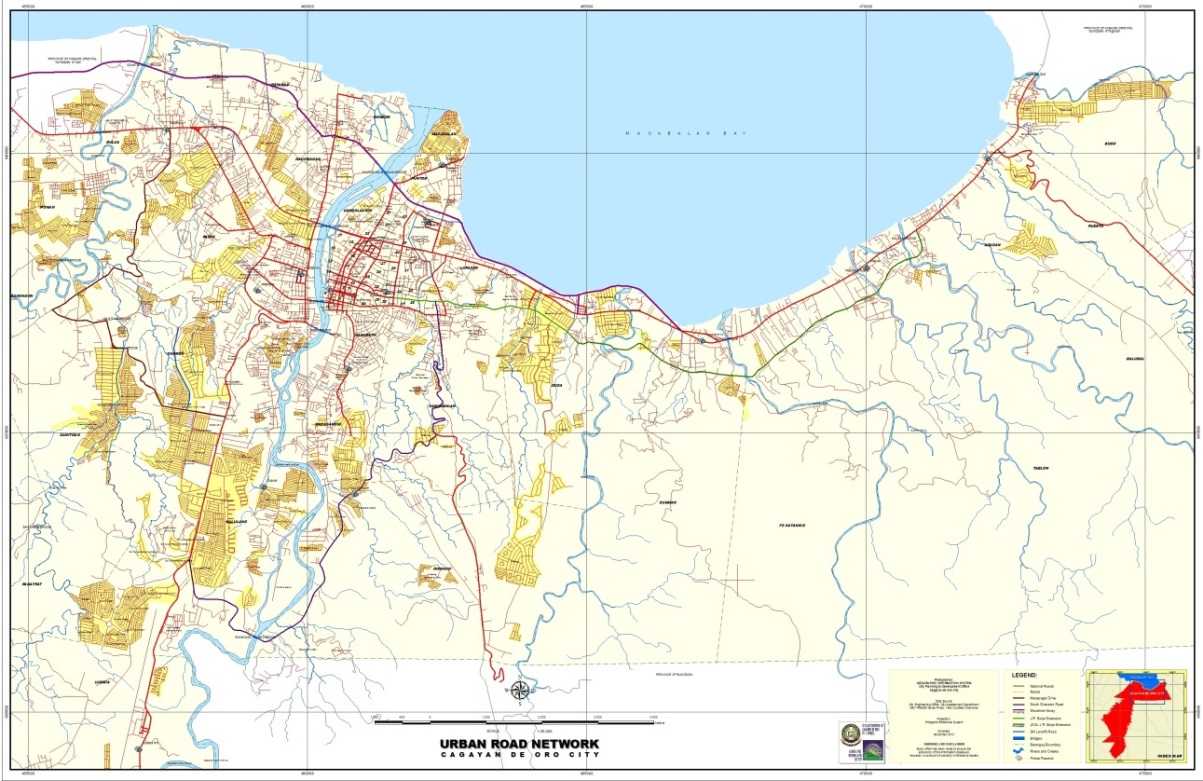
\includegraphics[width=0.85\textwidth, angle=0]{./scenarios/figures/philippines_fig1.png}}%
{GIS City Planning Office, 2012}

\createfigure%
{Spatial coverage of road network and locations of facilities in the network}%
{Spatial coverage of road network and locations of facilities in the network: it has 73.2\,square kilometers including land and surrounding river and coastal areas. The facilities are mapped based on its actual geographical x and y coordinates in the road network. There are 23\,facilities located in its nearest link in the network. These are: 10\,hospitals, three fire stations, eight police stations and two evacuation centers}%
{\label{fig:philippines_fig3}}%
{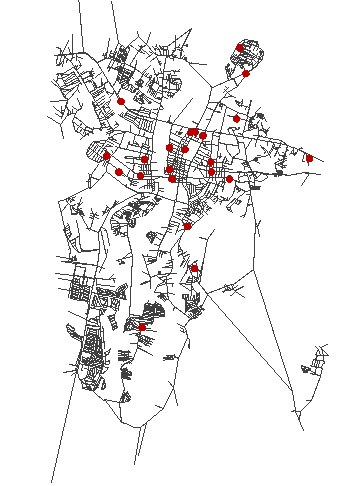
\includegraphics[width=0.85\textwidth, angle=0]{./scenarios/figures/philippines_fig3.png}}%
{}

\createfigure%
{Nodes and links representation}%
{Nodes and links representation: Road Network has 3\,837\,nodes representing road intersections and 9\,630\,links representing the streets. It includes five major bridges along Cagayan River: A. Kauswagan-Puntod Bridge, B. Maharlika Bridge (formerly known as Marcos Bridge), C.\ Gov.\ Ysalina Bridge (formerly known as Carmen Bridge), D. Kagay-an Bridge (Rotunda Bridge) and E. Emmanuel Pelaez Bridge}%
{\label{fig:philippines_fig2}}%
{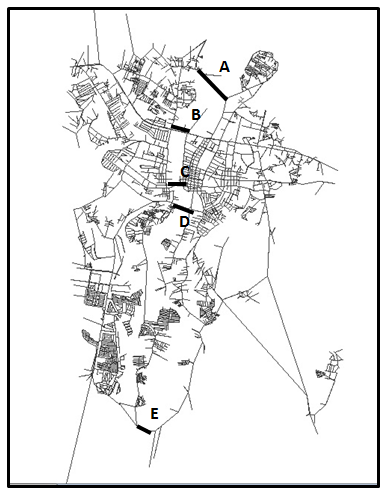
\includegraphics[width=0.85\textwidth, angle=0]{./scenarios/figures/philippines_fig2.png}}%
{}

\createfigure%
{Screenshot of SCENARIO~1}%
{Screenshot of SCENARIO~1 (without bridge closures) using agent~ID\#4. \protect\gls{drv} trip starting from the Sabal Hospital (Origin) passing Carmen Bridge (Gov. Ysalina Bridge) going to Balulang Evacuation Center dropping point (destination) then back to its origin}%
{\label{fig:philippines_fig4}}%
{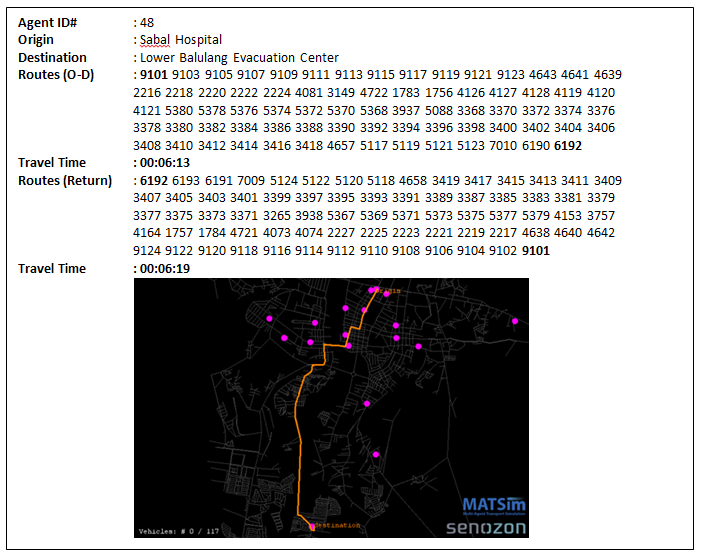
\includegraphics[width=0.85\textwidth, angle=0]{./scenarios/figures/philippines_fig4.png}}%
{}

\createfigure%
{Screenshot of SCENARIO~2}%
{Screenshot of SCENARIO~2 (with bridge closures) using agent~ID\#48. \protect\gls{drv} trip starting from the Sabal Hospital (Origin) passing Kauswagan-Puntod Bridge going to Balulang Evacuation Center dropping point (destination) then back to its origin}%
{\label{fig:philippines_fig5}}%
{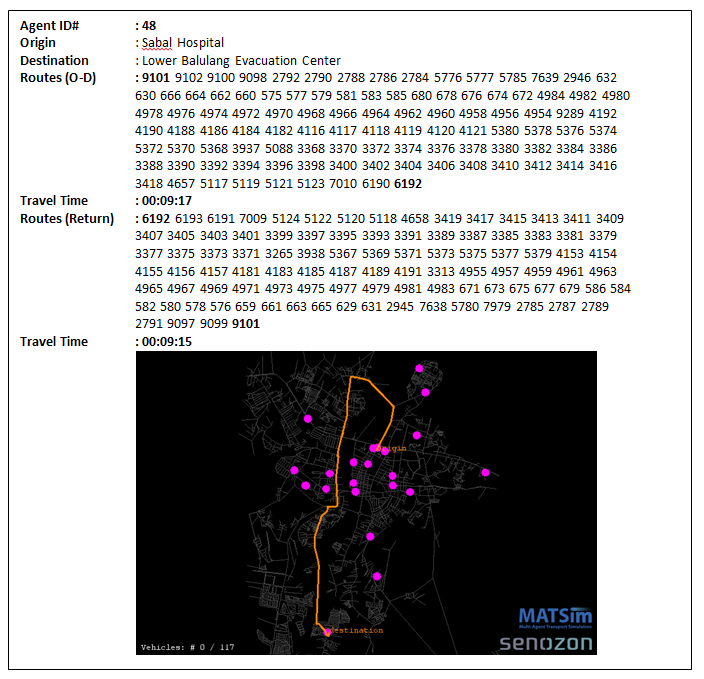
\includegraphics[width=0.85\textwidth, angle=0]{./scenarios/figures/philippines_fig5.png}}%
{}

% ##################################################################################################################






 
